\documentclass[12pt]{article}
\usepackage{bnpreport} % Required for inserting images

\title{Master Thesis}
\author{Jean Adrien LAGESSE}
\date{August 2023}

\begin{document}

\begin{titlepage}
   \begin{center}       
        \rule{1.1\textwidth}{1pt}
        \vspace{0.7cm}
        {\huge
        Over-smoothing and diffusion dynamics on graphs\\
        }
        \vspace{0.8cm}
        \textit{Master Thesis}
        \vspace{0.7cm}
        \rule{1.1\textwidth}{1pt}


       \vfill
            
        \begin{center}
            
\includegraphics[width=0.55\textwidth]{images/logo.png}
        \end{center}
       
       \vspace{3cm}
   \end{center}
   
   \textbf{University}: Imperial College London\\
    \textbf{Departement}: Mathematics\\
    \textbf{Supervisor}: Jeroen Lamb\\
    \textbf{Date}: September 2023\\
    \textbf{Student name}: Jean Adrien Lagesse\\
    \textbf{Student CID}: 02331224
\end{titlepage}

\newpage
\vspace{4cm}
\section*{\centering Abstract}
\vspace{1.5cm}
Over-smoothing is a recurrent problem when working with Graph Neural Networks that severely limits the expressiveness of well-known architectures. In this report we have gathered from different papers a mathematically tractable definition of this problem, we proposed a proof of the exponential over-smoothing of the isotropic diffusion equation on graphs and generalized it to anisotropic positive diffusion dynamics. To prove these theorems, we introduced different pseudo-Euclidean spaces adapted to measure over-smoothing in different use cases. Finally, we implemented a fast GPU-optimized algorithm based on the Graph Fourier transformation to analyze in practice this phenomenon for Erdos-Rényi random graphs.

\newpage
\section*{\centering Integrity statement on plagiarism }
The work contained in this thesis is my own work unless otherwise stated.

\section*{\centering Acknowledgment}
I would like to thank Professor Jeroen Lamb and Victoria Klein for their help and guidance.

\newpage
\section*{\centering Notations}
$\mathbf{G = (V,E)}$: A simple connected undirected graph with vertices set $\{1,...,V\}$ and edges in $\{1,...,V\}^2$.\\

$\mathbf{\mathcal{X}^l(G})$: The set of all l-dimensional signals on the vertices of the graph $G$, associating every vertex with a vector in $\mathbb{R}^l$.\\

$\mathbf{\mathcal{H}^l(G)}$: The set of all l-dimensional signals on the edges of the graph $G$, associating every edge with a vector in $\mathbb{R}^l$. The signals on $G$ are alternating: if $\epsilon \in \mathcal{H}^l(G)$ and $(i,j) \in E$,then $\epsilon(i,j) = - \epsilon(j,i)$.\\

$\mathbf{i \sim j}$: The vertices $i$ and $j$ are neighbours in $G$ (\textit{i.e.} $(i,j) \in E$).\\

$\mathbf{\bigoplus}$: Aggregation operator.\\

$\mathbf{A}$: Adjacency matrix of the graph $G$.\\

$\mathbf{\Delta}$: Laplacian of the graph $G$.\\

$\mathbf{\bar{\Delta}}$: Normalized Laplacian of the graph $G$.\\

$\mathbf{\Tilde{\Delta}}$: Normalized augmented Laplacian of the graph $G$.\\

$\mathbf{E_{\Delta}(X)}$: Dirichlet Energy associated with the Laplacian $\Delta$ of a signal $X \in \mathcal{X}^l(G)$ on the graph $G$.\\

$\mathbf{E_{\bar{\Delta}}(X)}$: Dirichlet Energy associated with the normalized Laplacian $\Delta$ of a signal $X \in \mathcal{X}^l(G)$\\

$\mathbf{E_{\Tilde{\Delta}}(X)}$: Dirichlet Energy associated with the augmented normalized Laplacian $\Delta$ of a signal $X \in \mathcal{X}^l(G)$ on the graph $G$.\\

$\mathbf{E_{S}(X)}$: Dirichlet Energy associated with the symmetric positive semi-definite matrix $S$ of a signal $X \in \mathcal{X}^l(G)$ on the graph $G$.\\

$\mathbf{<X,Y>} = tr(X^T Y)$: inner product on $\mathcal{X}^l(G)$\\

$\mathbf{\left| \left| X \right| \right|_2}$: $L^2$ vector norm.\\

$\mathbf{\left| \left| M \right| \right|_2}$: Matrix norm associated with the $L^2$ vector norm. $\left| \left| M \right| \right|_2 = \max_{\left| \left| X \right| \right|_2 = 1} \left| \left| MX \right| \right|_2$ \\

$\mathbf{<X,Y>_{S}} = tr(X^T S Y)$: pseudo inner product induced by a symmetric, positive, semi-definite matrix $S$.\\


$\mathbf{\left| \left| M \right| \right|_S}$: Matrix norm associated with the Dirichlet energy. $\left| \left| M \right| \right|_S = \sup_{E_S(X) = 1} E_S(MX)$ \\

$\mathbf{\widehat{X}}$: Graph Fourier Transform of a signal $X \in \mathcal{X}^l(G)$\\

$\mathbf{\widehat{M}}$: Graph Fourier Transform of the matrix $M$.\\

$\mathbf{\lambda_1 \leq ... \leq \lambda_V}$: Eigenvalues of the symmetric matrix $S$ order in ascending order. If which matrix $S$ is not clear, we write $\lambda_i(S)$.\\

$\mathbf{\lambda_{min}, \lambda_{max}}$: Smallest and largest eigenvalue of a symmetric matrix.\\

$\mathbf{\dot{X}(t)}$: time derivative of $X$

\newpage
\tableofcontents

\newpage
\section{Introduction}

With the fast rise of Machine Learning finding new architectures that work for new data types has been a priority. The classical data types have always been Euclidean: text data can be seen as a 1-dimensional, images are 2-dimensional, etc... Yet, for many problems, Euclidean data types are not very well suited. Graphs being a very well-known and powerful data structure in computer science it was very natural to use it in several problems. The paper \mycite{gnn} presented the Graph Neural Network architecture. Since then, improving the original Graph Neural Network architecture has been a problem that many researchers are working on.\\

In the past few years, hundreds of different architectures for Graph Neural Networks have been presented, most of them can be classified into three categories:
\begin{enumerate}
    \item Graph Convolution Network: These architectures can be seen as a generalization of the Convolution Neural Networks used mainly in Computer Vision to Graphs. They are based on an approximation of  convolutions on graphs \mycite{gcn}.

    \item Graph Attention Networks: These architectures can be seen as a generalization of the transformers used mainly in Natural Language Processing to graphs \mycite{gat}.

    \item Message Passing Neural Networks: A strictly more powerful architecture than the Graph Attention Network \mycite{mpnn}.
\end{enumerate}

The evolution of Graph Neural Networks closely follows the rest of the Machine Learning field. Several ideas first implemented in Computer Vision and Natural Language processing have been implemented in Graph Neural Networks. In this report, we are particularly interested in the Residual Connection Networks paper \mycite{resnet} that was later used to define the Neural Ordinary Differential Equation Network architecture \mycite{neuralodenet} and enables the use of continuous-time processes as Neural Networks. These two papers enable us to consider the discrete layers of a Graph Neural Network as a continuous function which simplifies the study of the dynamics on the graph.

\newpage

\section{Graph Neural Network}

\subsection{Graphs and signals on graphs}
Let's consider a graph $G =(V,E)$ where the vertices are numbered from $1$ to $V$ and where the edges in $E$ are the pairs $(i,j)$ for some $(i, j) \in \{1,...,V\}^2$, moreover we consider that the graph is simple, undirected and connected.\\

On this graph $G$, we will assign features to each vertex, those features are vectors of a fixed size $l$, hence, we can represent all the features of the graph as a $V \times l$ matrix that we will call $X$. We say that $X$ is an l-dimensional signal on $G$ and we call $\mathcal{X}^l(G)$ the set of all l-dimensional signals.\\

Similarly, we can assign features to the edges of $G$. Let $\epsilon: \{1,...,V\}^2 \longrightarrow \mathbb{R}^l$ such that for all $(i,j) \in \{1,...,V\}^2$, $\epsilon(i,j) = - \epsilon(j,i)$, and such that if $(i,j) \not\in E$ then $\epsilon(i,j) = 0$. We say that $\epsilon$ is an l-dimensional edge signal on $G$ and we call $\mathcal{H}^l(G)$ the set of all l-dimensional edge signals.

\subsection{Architecture}

In the most general definition, a graph neural network is a function $H_{\theta}$ parameterized by $\theta$, that takes as input a graph $G$ with an $l_{in}$-dimensional signal $X_{in}$ and outputs an $l_{out}$-dimensional signal. Moreover, the function $H_{\theta}$ should be able to take any graph $G$ as its input but we will require that $l_{in}$ and $l_{out}$ (the number of features we have per vertices) stay the same.\\

A graph neural network is a type of Neural Network that takes as an input a graph and gives back another graph. A key element of Graph Neural Networks is that the same network can be used on graphs of different structures and different sizes, whereas classical neural networks have a fixed vector size as an input. This is very useful when working on heterogeneous data such as molecules: each molecule has a different number of atoms and covalent bonds, making it very hard to have a fixed vector size representation.\\

\subsection{Optimization and training of a Graph Neural Network}
Let's consider that we have a training set $\mathbb{X} = (G_i,X_i)_{i \in \{1,...,N\}}$ consisting of $N$ graphs and $N$ $l_{in}$-dimensional signals. Moreover, we have $\mathbb{Y} = (G_i,Y_i)_{i \in \{1,...,N\}}$ consisting of $N$ graphs and $N$ $l_{out}$-dimensional signals. Our aim is to find the optimal $\theta^*$ such that $H_{\theta^*}$ predict for each $i \in  \{1,...,V\}$ $Y_i$ from $X_i$. In practice, we try to solve:
\begin{align}\label{fn:optimization}
    \theta^* = \argmin_{\theta} \sum_{i = 1}^N \mathcal{L}(H_{\theta}(X_i, G_i), Y_i) + \mathcal{L}_{reg}(\theta)
\end{align}

where $\mathcal{L}$ is a loss function and $\mathcal{L}_{reg}$ is a regularization  penalty.\\

When the function $H_{\theta}$ is differentiable, the usual choice to find an approximate solution of \ref{fn:optimization} is to use the stochastic gradient descent algorithm.

\subsection{Aggregation function}

 The most important requirement is that our function $H$ work on a graph of any structure {\it i.e.} with a different number of vertices and different edges, moreover we want to use this structure as it carries information about the data on which we are working. Intuitively, we want to learn the output feature of a vertex by analyzing its neighbourhood in the graph; to be able to extract this information, we need an {\it aggregation function}, this function will take an arbitrary number of neighbours of a vertex and aggregate it into a fixed size vector, in the rest of the report, this aggregation function will be denoted as $\bigoplus$, and will aggregate any number of feature vector $\{v_1,...,v_m\}$ into another vector $\bigoplus_{i=1}^m v_i$. To make sense, the {\it aggregation function} must be invariant under permutation because there is no canonical order of vertices in a graph, hence for a permutation $\sigma$, we must have that $\bigoplus_{i=1}^m v_i = \bigoplus_{i=1}^m v_{\sigma(i)}$. This function will compute a {\it representation} of the neighbourhood of a vertex. Let $\{v_1,...,v_m\}$ be vectors in $\mathbb{R}^l$, here are a few examples of {\it aggregation functions}:
\begin{itemize}
    \item $\bigoplus_{i=1}^m v_i = \dfrac{1}{m} \sum_{i=1}^m v_i$
    \item $\bigoplus_{i=1}^m v_i = (max(v_1[1],...,v_m[1]),..., max(v_1[l],...,v_m[l])^T$
    \item $\bigoplus_{i=1}^m v_i = (min(v_1[1],...,v_m[1]),..., min(v_1[l],...,v_m[l])^T$
\end{itemize}

\subsection{Building a Graph Neural Network by stacking layers}

\noindent Now that we have defined the aggregation function, we can give a general formula for the function $H$. Let's consider $l_{input} = l_0, l_1,...,l_N = l_{output}$ the dimension of the input signal, output signal and intermediate signals that we will use. We will also break down the function $H$ in several layers such that $H = h_0 \circ ... \circ h_{N-1}$, where each layer $h_i$ will take as an input the graph $G$ and it's $l_i$-dimensional signal $X_i \in \mathcal{X}^l_i(G)$ and output a new $l_{i+1}$-dimensional signal $X_{i+1} \in \mathcal{X}^l_{i+1}(G)$
\\

\noindent Now we will give the general formula for each layer, let's consider the layer $h_k$ that takes as an input $X_{k}$ and outputs $X_{k+1}$, we will denote $x_j^{(k)}$ the feature vector associated with the $j^{th}$ vertices in  $X_k$. The function $h_k$ is composed of two parameterized functions $\gamma^{(k)}$ and $\phi^{(k)}$ (usually {\it multi-layer perceptrons}) and we can compute the new signal $X_{k+1}$ with the following formula:
$$
x_i^{(k+1)} = \gamma^{(k)}(x_i^{(k)}, \bigoplus_{j \sim i} \phi^{(k)} (x_i^{(k)}, x_j^{(k)}))
$$

\begin{figure}[h]
\centering
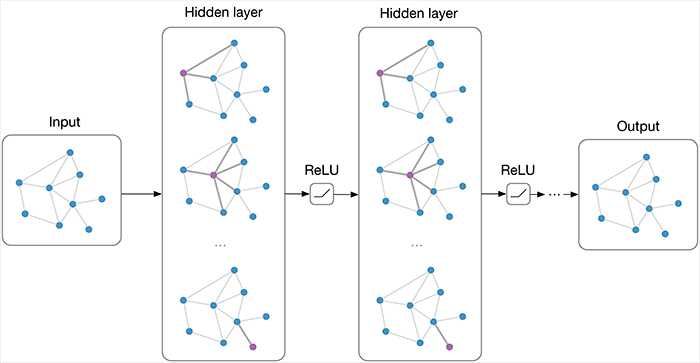
\includegraphics[width=1.0\textwidth]{images/gnn-image.jpeg}
\caption{Visualization of the layers of a Graph Neural Network: We can see a graph $G$ with a feature matrix of dimension $V \times l_i$ as $l_i$ graph with a feature matrix of dimension $V \times 1$, each of these graph represents a different learned information. (source: Thomas Kipf - Deep learning with graph-structured representations)}
\end{figure}


\subsection{Classification of Graph Neural Network architectures}
In the literature, many different Graph Neural Networks architectures have been presented, however most of them can be classified in the following way:

\begin{definition}[The expressive power of Graph Neural Networks].\\
    \begin{itemize}
        \item \textbf{Convolution Graph Neural Networks}: this architecture is the simplest and is described by the following equation for each layer:
        $$
        x_i^{(k+1)} = \gamma^{(k)}(x_i^{(k)}, \bigoplus_{j \sim i} H_{i,j}  x_j^{(k)})
        $$
         {\it N.B}: $H$ a matrix.
        \item \textbf{Graph Attention Networks}: this architecture is in between the Convolution Graph Neural Network and the Message Passing Neural Network, rather than simply aggregating the features, we will perform a weighted aggregation:
        $$
        x_i^{(k+1)} = \gamma^{(k)}(x_i^{(k)}, \bigoplus_{j \sim i} a^{(k)} (x_i^{(k)}, x_j^{(k)}) x_j^{(k)})
        $$
        {\it N.B}: The function $a^{(k)}$ compute a weight in $\mathbb{R}$.
        \item \textbf{Message Passing Neural Networks}: this architecture is the more general and the more expressive, for each pair of features we will compute a completely new feature to be aggregated. It is the same equation as in the previous section:
        $$
        x_i^{(k+1)} = \gamma^{(k)}(x_i^{(k)}, \bigoplus_{j \sim i} \phi^{(k)} (x_i^{(k)}, x_j^{(k)}))
        $$
    \end{itemize}
\end{definition}

Each one of those architectures or more powerful than the previous one, however, this complexity comes at a cost. Indeed, as the neural network gets more expressive, it is harder to train. Nevertheless, depending on the characteristics of the data on which we are working, using a more expressive model can be required.

\subsection{From discrete layers to continuous layers}

Residual Networks \mycite{resnet} were first introduced in Computer Vision to have a better propagation of the gradient in the Neural Network (useful for the stochastic descent algorithm). Applying this to Graph Neural Networks means to parameterize differently the layer-wise equation:
$$
        x_i^{(k+1)} = x_i^{(k)} +\gamma^{(k)}(x_i^{(k)}, \bigoplus_{j \sim i} \phi^{(k)} (x_i^{(k)}, x_j^{(k)}))
$$

In \textit{Neural Ordinary Differential Equations }\mycite{neuralodenet}, it was suggested that for Residual Networks, it is possible to consider that the Neural Network layers are continuous. Applying this to the Graph Neural Network architecture yields to the following differential equation:


\begin{equation}\label{graphode}
    \dot{x}_i(t) = \gamma(t)(x_i(t), \bigoplus_{j \sim i} \phi(t)( (x_i(t), x_j(t)))
\end{equation}

With this formalism $t \mapsto \gamma(t)$ and $t \mapsto \phi(t)$ assigns to each $t$ a parameterized function. Ways to build and optimize those function are presented in \mycite{neuralodenet} but are not relevant to the rest of this report.\\

The equation \ref{graphode} is linked to the Message Passing Neural Network update equation by the Euler discretization scheme, for $\tau = 1$ we have:

\begin{align*}
    \dfrac{x_i(t+\tau) - x_i(t)}{\tau} = \gamma(t)(x_i(t), \bigoplus_{j \sim i} \phi(t)( (x_i(t), x_j(t))) \\\\
    x_i(t+\tau) = x_i(t) + \tau \gamma(t)(x_i(t), \bigoplus_{j \sim i} \phi(t)( (x_i(t), x_j(t)))\\\\
    x_i(t+1) = x_i(t) + \gamma(t)(x_i(t), \bigoplus_{j \sim i} \phi(t)( (x_i(t), x_j(t)))
\end{align*}

Hence, we can see that discrete and continuous layers follow the same dynamics when the number of layers is big (\textit{i.e.} when $\tau$ is small).


\newpage
\section{Properties and limitations of Graph Neural Networks}

\subsection{Importance of deep Graph Neural Networks}

Deep Learning is a sub-field of Machine Learning where several layers are stacked one after each other, using deep learning enables learning very complex relationships in the data and has resulted in state-of-the-art methods in several domains such as Computer Vision and NLP. Empirically, it has been shown that large and deep models perform better than shallow models. Large Language Models consist of tens of layers \mycite{llama} and image recognition architectures can rise to hundreds of layers \mycite{resnet}.\\

In Graph Neural Networks, having many layers has another important role:

\begin{thm}
    Consider a Graph Neural Network with $N$ layers, the output feature of a vertex $v$ depends exactly on the features of all the vertices at a distance of $N$ or less to $v$.
\end{thm}

Hence, to be able to learn interactions between long-distance vertices, it is necessary to have very deep Graph Neural Networks. However, several problems arise when considering deep GNN architectures. We will investigate those problems by considering the dynamics on the graph in the following parts of the report.

\subsection{Limitations of deep Graph Neural Networks}

\begin{definition}
    Graphs can be classified in two main categories:
    \begin{itemize}
        \item \textbf{Homophilic graphs}: We call a graph homophilic if we expect that neighboring vertices will share the same features. An example of such graphs is social media graphs: if two persons are friends on a social network (\textit{i.e} are neighbors in the friendship graph) we can expect that they will share the same features such as location, political views, etc...

        \item  \textbf{Heterophilic graphs}: We call a graph heterophilic if we expect that neighboring vertices don't share the same features. An example of such graphs is the graph representation of a molecule (\textit{i.e} the graph where vertices are atoms and edges represent the covalent bonds), indeed, in molecules, very different atoms share covalent bonds hence they will have different features.
    \end{itemize}
\end{definition}

\begin{figure}[h]
\centering
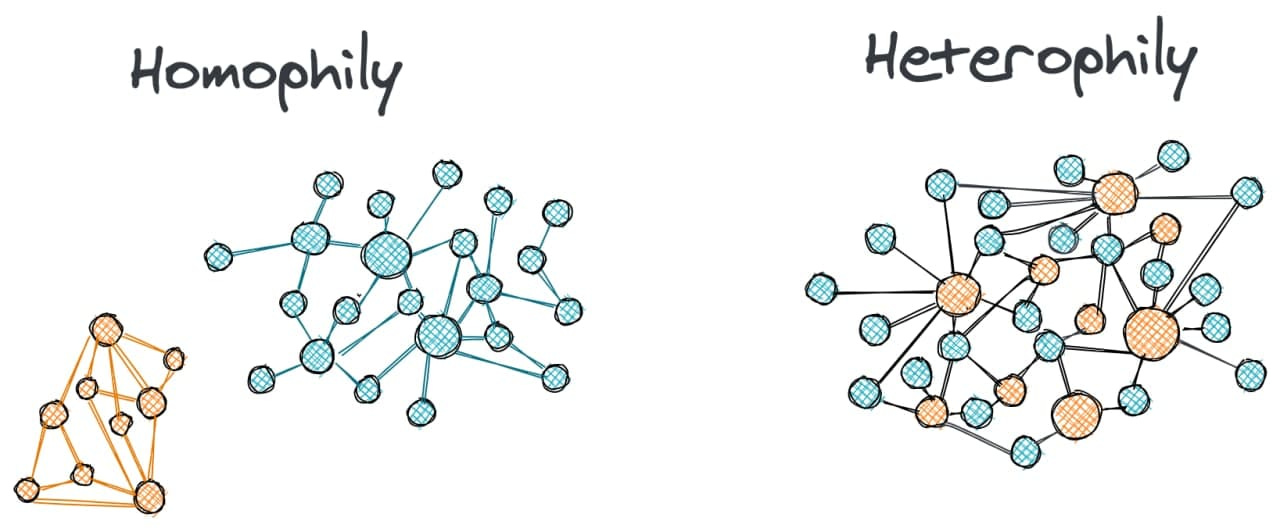
\includegraphics[width=0.9\textwidth]{images/homophilyVSheterophily.jpeg}
\caption{Visualization of heterophilic and homophilic graphs. \\(source: https://graphml.substack.com/p/gml-newsletter-homophily-heterophily)}
\end{figure}

 On homophilic graphs simple models such as a Graph Convolutional Network can yield very good results, however, on heterophilic graphs, the neural network cannot distinguish vertices that are similar to one another from the ones that should share very different features, hence, during the aggregation step all this information is lost and this yields to an output graph that is very smooth (neighboring nodes are very similar): that problem is commonly known as \textbf{over-smoothing}.
\\


\begin{figure}[h!]
\centering
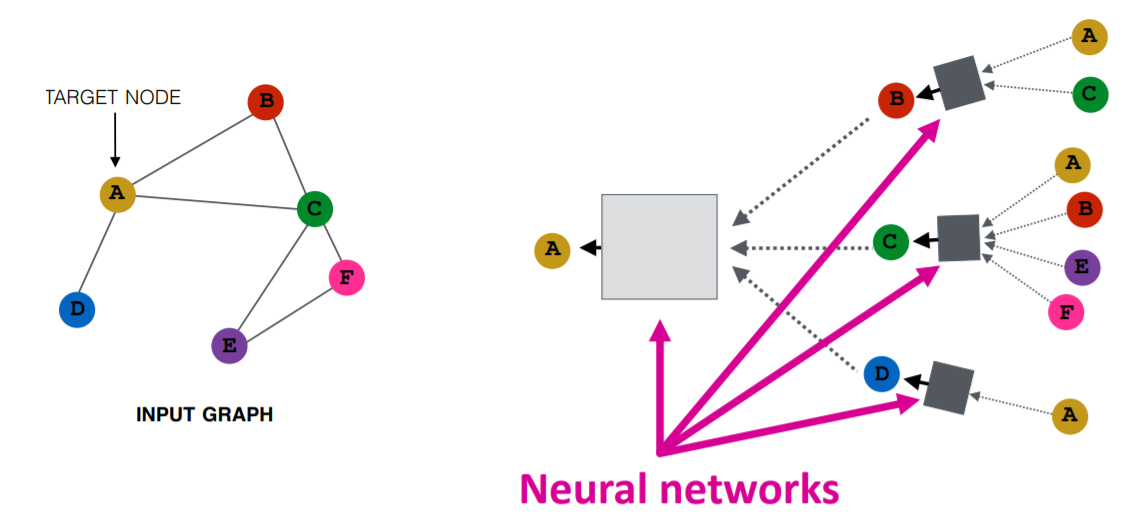
\includegraphics[width=0.7\textwidth]{images/gnn-unwinding.png}
\caption{Unwinding of the layers of a Graph Neural Network from the point of view of a single vertex. (source: https://medium.com/neuralspace/graphs-neural-networks-in-nlp-dc475eb089de)}
\label{fig:gnnunwinding}
\end{figure}

Over-smoothing can also arise from very deep Graph Neural Networks, as seen in \ref{fig:gnnunwinding}, the vertices present when unwinding the Graph Neural Network are often repeated, hence when we have many layers, the information learned about a vertex is nearly the same as the its neighbours, resulting in over-smoothing.
\\

 In addition to over-smoothing, another well know problem when using Graph Neural Network is \textbf{bottlenecks}. As we can see in \ref{fig:gnnunwinding}, with only a few layers and a few neighbouring vertices, the information that a vertices contains is very packed, which means that it is very hard for the neural network to use all the available information, this can become quite a problem when there are very few edges connecting different dense part of the graph, just as shown in \ref{fig:bottlenecks}.

\begin{figure}[h!]
\centering
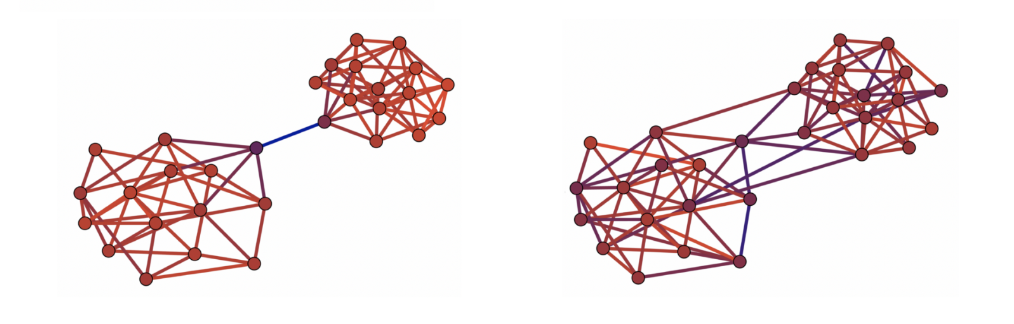
\includegraphics[width=0.9\textwidth]{images/bottlenecks.png}
\caption{On the left we can see that a bottleneck will appear, information will difficultly flow between the right and left part of the graph. On the graph on the right, because there is more edges connecting the two parts, the information will be able to flow. (source: https://blog.twitter.com/engineering)}
\label{fig:bottlenecks}
\end{figure}

\newpage
\section{Spectral Graph Theory and Dirichlet Energy}

To study Graph Convolution Networks and to prove that they are subject to over-smoothing, we will need the formalism of Graph Spectral Theory, a subset of graph theory that studies the relationships between the eigenvalues of the graph Laplacian and properties of the graph. Most of the definitions are inspired by \mycite{gst}, however, based on the formula we used for the graph Laplacian, different properties emerge.\\

In addition, we define a new pseudo-Euclidean space that is adapted to study the Dirichlet energy of a graph. As we will see, the Dirichlet energy is linked to the Laplacian and we generalize the definition of the Dirichlet Energy to other types of graph Laplacians.


\subsection{Common definitions}

Let $G = (V, E)$ be a simple connected undirected graph.

\begin{definition}[Adjacency matrix]
    The adjacency matrix of $G$ is a matrix $A \in \mathcal{M}_{V \times V}(\{0,1\})$ such that for $i,j \in \{1,...,V\}$, $A_{i,j} = 1$ if and only is $(i,j) \in E$ and $A_{i,j} = 0$ otherwise.\\
    
    The augmented adjacency matrix of $G$ is $\Tilde{A} = A + \mathbb{I}d \in \mathcal{M}_{V \times V}(\{0,1\})$. It is the adjacency matrix of $G$ augmented with self-loops.
\end{definition}

\begin{definition}[Degree matrix]
    The degree matrix of $G$ is the diagonal matrix $D=diag(d_1,...,d_V) \in \mathcal{M}_{V \times V}(\mathbb{N})$.\\
    
    The augmented degree matrix of $G$ is the diagonal matrix  $\Tilde{D}= diag(d_1+1,...,d_V+1) = D + \mathbb{I}d \in \mathcal{M}_{V \times V}(\mathbb{N})$. It is the degree matrix of $G$ augmented with self-loops.
\end{definition}

\begin{definition}[Graph Laplacian]
    The graph Laplacian of $G$ is the matrix $\Delta = D - A$.\\

    The normalized graph Laplacian of $G$ is the matrix $\bar{\Delta} = D^{-\frac{1}{2}}(D - A)D^{\frac{1}{2}}$\\
    
    The augmented normalized graph Laplacian of $G$ is the matrix
    \begin{align*}
        \Tilde{\Delta} &= \Tilde{D}^{-\frac{1}{2}} \Delta \Tilde{D}^{-\frac{1}{2}} \\
        &= \Tilde{D}^{-\frac{1}{2}}(\Tilde{D} - \Tilde{A}) \Tilde{D}^{-\frac{1}{2}} \\
        &= \mathbb{I}d - \Tilde{D}^{-\frac{1}{2}}\Tilde{A} \Tilde{D}^{-\frac{1}{2}}
    \end{align*}
\end{definition}

To have a a better intuition of how these operators act on a signal we can
consider a 1-dimensional signal $X \in \mathbb{R}^V$on the graph $G$ and let $i \in \{1,...,V\}$ be a vertex of $G$:
\begin{align*}
    \Delta(X)_i &= (DX)_i - (AX)_i \\
                &= d_i x_i - \sum_{j \sim i} x_j \\
                &= \sum_{j \sim i} x_i - x_j
\end{align*}

From that formula we can deduce:

\begin{align*}
    \bar{\Delta}(X) &= \bar{D}^{-\frac{1}{2}} \Delta \bar{D}^{-\frac{1}{2}} X \\
    &= \bar{D}^{-\frac{1}{2}} \Delta (\frac{x_i}{\sqrt{d_i}})_{i \in \{1,...,V\}} \\
    &= \bar{D}^{-\frac{1}{2}} (\sum_{j \sim i} \frac{x_i}{\sqrt{d_i}} - \frac{x_j}{\sqrt{d_j}})_{i \in \{1,...,V\}} \\
    &= (\frac{1}{\sqrt{d_i}} \sum_{j \sim i} \frac{x_i}{\sqrt{d_i}} - \frac{x_j}{\sqrt{d_j}})_{i \in \{1,...,V\}}
\end{align*}
and also:
\begin{align*}
    \Tilde{\Delta}(X) &= \Tilde{D}^{-\frac{1}{2}} \Delta \Tilde{D}^{-\frac{1}{2}} X \\
    &= \Tilde{D}^{-\frac{1}{2}} \Delta (\frac{x_i}{\sqrt{d_i +1}})_{i \in \{1,...,V\}} \\
    &= \Tilde{D}^{-\frac{1}{2}} (\sum_{j \sim i} \frac{x_i}{\sqrt{d_i +1}} - \frac{x_j}{\sqrt{d_j +1}})_{i \in \{1,...,V\}} \\
    &= (\frac{1}{\sqrt{d_i +1}} \sum_{j \sim i} \frac{x_i}{\sqrt{d_i +1}} - \frac{x_j}{\sqrt{d_j +1}})_{i \in \{1,...,V\}}
\end{align*}


\subsection{Properties of the Laplacian}
\begin{thm}\label{thm:laplacian}
    $\Delta$, $\bar{\Delta}$ and $\Tilde{\Delta}$ are symmetric, positive semi-definite matrices.
\end{thm}

\begin{proof}\label{thm:laplacianmatrix}
    The matrix $D$ is diagonal hence it is symmetric, moreover, because $G$ is undirected, if $(i,j) \in E$ then $(j,i) \in E$, hence $A$ is symmetric. This proves that $\Delta$ is symmetric.\\
    In addition it is clear that $\bar{D}^{-\frac{1}{2}}$ and $\Tilde{D}^{-\frac{1}{2}}$ are diagonal, so we can say that they are symmetric. Hence:
    \begin{equation*}
        \bar{\Delta}^T = (\bar{D}^{-\frac{1}{2}} \Delta \bar{D}^{-\frac{1}{2}})^T = (\bar{D}^{-\frac{1}{2}})^T \Delta^T (\bar{D}^{-\frac{1}{2}})^T = \bar{\Delta}
    \end{equation*}
    \begin{equation*}
        \Tilde{\Delta}^T = (\Tilde{D}^{-\frac{1}{2}} \Delta \Tilde{D}^{-\frac{1}{2}})^T = (\Tilde{D}^{-\frac{1}{2}})^T \Delta^T (\Tilde{D}^{-\frac{1}{2}})^T = \Tilde{\Delta}
    \end{equation*}
    Now, let $X = (x_i)_{i \in \{1,...,V\}}$ be a 1-dimensional signal on $G$:
    \begin{align*}
        X^T \Delta X &= \sum_{i=1}^V x_i \sum_{j \sim i} x_i-x_j \\
                    &= \sum_{i,j =1}^V A_{i,j} x_i^2 - x_i x_j \\
                    &= \sum_{i,j = 1}^V A_{i,j} \frac{1}{2}(x_i -x_j)^2 + \frac{1}{2}(x_i^2 -x_j^2) \\
                    &= \frac{1}{2} \sum_{i,j = 1}^V A_{i,j} (x_i -x_j)^2 \geq 0
    \end{align*}
    Based on this result, a same result can be found for $\bar{\Delta}$ and $\Tilde{\Delta}$:
    \begin{align*}
     X^T \bar{\Delta} X &= X^T\bar{D}^{-\frac{1}{2}} \Delta \bar{D}^{-\frac{1}{2}}X = (\bar{D}^{-\frac{1}{2}} X)^T \Delta (\bar{D}^{-\frac{1}{2}}X) \\
        &= \frac{1}{2} \sum_{i,j = 1}^V A_{i,j} (\frac{x_i}{\sqrt{d_i}} -\frac{x_j}{\sqrt{d_j}})^2 \geq 0\\\\
        X^T \Tilde{\Delta} X &= X^T\Tilde{D}^{-\frac{1}{2}} \Delta \Tilde{D}^{-\frac{1}{2}}X = (\Tilde{D}^{-\frac{1}{2}} X)^T \Delta (\Tilde{D}^{-\frac{1}{2}}X) \\
        &= \frac{1}{2} \sum_{i,j = 1}^V A_{i,j} (\frac{x_i}{\sqrt{d_i+1}} -\frac{x_j}{\sqrt{d_j+1}})^2 \geq 0
    \end{align*}

    \noindent Hence, $\Delta$, $\bar{\Delta}$ and $\Tilde{\Delta}$ are semi-definite, however, we can prove that they are not definite by considering $X= (1)_{i \in \{1,...,V\}}$ for $\Delta$, $X = (\sqrt{d_i})_{i \in \{1,...,V\}}$ for $\bar{\Delta}$ and $X = (\sqrt{d_i +1})_{i \in \{1,...,V\}}$ for $\Tilde{\Delta}$.
\end{proof}



\begin{thm} \label{thm:laplacianeigenvalues}
    The eigenvalues of $\bar{\Delta}$ are in $[0,2]$ and the eigenvalues of $\Tilde{\Delta}$ are in $[0,2)$
\end{thm}

\begin{proof}
    Because $\bar{\Delta}$ and $\Tilde{\Delta}$ are positive semi-definite (Theorem \ref{thm:laplacianmatrix}), every eigenvalues are greater than $0$. Now, let $X$ be a 1-dimensional signal on $G$ such that $||X||_2 = 1$, then:
    \begin{align*}
        X^T \bar{\Delta} X  &= \frac{1}{2} \sum_{i,j = 1}^V A_{i,j} (\frac{x_i}{\sqrt{d_i}} -\frac{x_j}{\sqrt{d_j}})^2 \\
        &\leq  \sum_{i,j = 1}^V A_{i,j}(\frac{x_i^2}{d_i} + \frac{x_j^2}{d_j}) \\
        &= \sum_{i=1}^V x_i^2 + \sum_{j=1}^V x_j^2 \leq 2
    \end{align*}
    
    \begin{align*}
        X^T \Tilde{\Delta} X  &= \frac{1}{2} \sum_{i,j = 1}^V A_{i,j} (\frac{x_i}{\sqrt{d_i+1}} -\frac{x_j}{\sqrt{d_j+1}})^2 \\
        &\leq  \sum_{i,j = 1}^V A_{i,j}(\frac{x_i^2}{d_i+1} + \frac{x_j^2}{d_j+1}) \\
        &= \sum_{i=1}^V \frac{d_i}{d_i +1} x_i^2 + \sum_{j=1}^V \frac{d_j}{d_j+1} x_j^2 < 2
    \end{align*}

    Let $\lambda$ be the largest eigenvalue of $\bar{\Delta}$, and let $X$ be the associated eigenvector, then $X^T \bar{\Delta} X = \lambda X^T X = \lambda \leq 2$.\\

     Let $\lambda$ be the largest eigenvalue of $\Tilde{\Delta}$, and let $X$ be the associated eigenvector, then $X^T \Tilde{\Delta} X = \lambda X^T X = \lambda < 2$.
\end{proof}

\begin{definition}[Pseudo inner-product]
    Let a $S$ be a symmetric positive semi-definite matrix, the mapping $<,>_{S}: (X,Y) \in \mathcal{X}^l(G)^2 \longmapsto tr(X^T S Y) \in \mathbb{R}$ is the  pseudo inner-product associated with the matrix $S$.
\end{definition}

\begin{thm}
    Pseudo inner-product associated with the matrix $S$ is indeed a pseudo inner-product.
\end{thm}

\begin{proof}
    Let $X,Y,Z$ be l-dimensional signal on $G$, then:
    \begin{itemize}
        \item \textbf{Symmetry}: $$<X,Y>_{S} = tr(X^T S Y) = tr((X^T S Y)^T) = tr(Y^T S X) = <Y,X>_{S}$$

        \item \textbf{Linearity}: Let $a,b \in \mathbb{R}$, then:
        \begin{align*}
            <aX+bY,Z>_{S} &= tr((aX+bY)^T S Z) = a\times Tr(X^T S Z) + b \times Tr(Y^T S Z) \\
            &=a<X,Z>_{S} +b<Y,Z>_{S}
        \end{align*}

        \item \textbf{Positive semi-definiteness}: 
        By applying the fact that $S$ is a positive semi-definite matrix it follows that:
        \begin{align*}
            <X,X>_{S} = tr(X^T S X) = \sum_{k=1}^V tr(X_{.,k}^T S X_{.,k}) \geq 0
        \end{align*}
    \end{itemize}
\end{proof}

By combining the definition of the pseudo inner product associated with a symmetric, positive, semi-definite matrix and the results from theorem \ref{thm:laplacian}, we can consider in the rest of the report the following pseudo inner products: $<.,.>_{\Delta}$, $<.,.>_{\bar{\Delta}}$ and $<.,.>_{\Tilde{\Delta}}$.\\

Hence we have defined on $\mathcal{X}^l(G)$ three different pseudo-Euclidean structures. We will prove that those spaces are very different but that they are useful for studying different measures of over-smoothing on a graph.


\subsection{Fourier Transform on Graphs}

It will be useful in the rest of the paper to be able to perform the Fourier transform of a signal $X \in \mathcal{X}^l(G)$ associated with $S \in \{\Delta, \bar{\Delta}, \Tilde{\Delta}\}$ . By theorem \ref{thm:laplacianeigenvalues}, we know that the eigenvalues of $S$ are positive, hence we can order them:
$$0= \lambda_1 \leq ... \leq \lambda_V $$
In \mycite{gst}, it is proved that $\lambda_2 = 0$ if and only if $G$ is not connected, hence $\lambda_2 > 0$ in our case.\\

There exist a square matrix $P$ such that  $S = P^{-1} diag(\lambda_1,..., \lambda_V) P $.

\begin{definition}[Fourier transform on graphs]
    If $X$ is a l-dimensional signal on $G$, the Fourier transform of $X$ is:
    $$
    \widehat{X} = P X
    $$
\end{definition}

The Fourier transform is build so that the following diagram is commutative:

\[ \begin{tikzcd}[row sep=huge, column sep=huge]
\mathcal{X}^l(G) \arrow{r}{S} \arrow[swap]{d}{P} & \mathcal{X}^l(G) \\%
\widehat{\mathcal{X}}^l(G) \arrow[swap]{r}{diag(\lambda_1,...,\lambda_V)}& \widehat{\mathcal{X}}^l(G) \arrow[swap]{u}{P^{-1}}
\end{tikzcd}
\]

\begin{definition}
    Let $M: \mathcal{X}^l(G) \mapsto \mathcal{X}^l(G)$, then the Fourier transform of $M$ is $\widehat{M} = P\circ M \circ P^{-1}$. In particular, if $M$ is a squared matrix of dimension $V$, $\widehat{M} = P M P^{-1}$
\end{definition}

This definition assures us that applying $M$ in $\mathcal{X}^l(G)$ is equivalent to applying $\widehat{M}$ in $\widehat{\mathcal{X}}^l(G)$. Let $X \in \mathcal{X}^l(G)$, then:
$$
\widehat{M}\widehat{X} = P\circ M \circ P^{-1} P X = P M X = \widehat{MX}
$$

\subsection{Dirichlet Energy}

\begin{definition}[Dirichlet Energy]
    Let $X \in \mathcal{M}_{V \times l}(\mathbb{R})$ be a l-dimensional signal on the graph $G$. The Dirichlet energy of $X$ associated with $\Delta$, $\bar{\Delta}$ or $\Tilde{\Delta}$ are:
    \begin{align*}
    E_{\Delta}(X) &= \sqrt{\frac{1}{2} \sum_{i,j = 1}^V A_{i,j} \left|\left|X_i -X_j\right|\right|_2^2 }\\\\
     E_{\bar{\Delta}}(X) &= \sqrt{\frac{1}{2} \sum_{i,j = 1}^V A_{i,j} \left|\left|\frac{X_i}{\sqrt{d_i}} -\frac{X_j}{\sqrt{d_j}}\right|\right|_2^2 }\\\\
        E_{\Tilde{\Delta}}(X) &= \sqrt{\frac{1}{2} \sum_{i,j = 1}^V A_{i,j} \left|\left|\frac{X_i}{\sqrt{d_i+1}} -\frac{X_j}{\sqrt{d_j+1}}\right|\right|_2^2 }
    \end{align*}
\end{definition}

\begin{thm}
    The Dirichlet energy associated with $S \in \{\Delta, \bar{\Delta}, \Tilde{\Delta}\}$ is the pseudo norm associated to $<.,.>_{S}$
\end{thm}

\begin{proof}
    \begin{align*}
        E_{\Delta}(X)^2 &= \frac{1}{2} \sum_{i,j = 1}^V A_{i,j} \left| \left|X_i-X_j \right| \right|_2^2 \\
        &= \frac{1}{2} \sum_{i,j = 1}^V A_{i,j} \sum_{k=1}^V x_{i,k}-x_{j,k})^2 \\
        &= \sum_{k=1}^V (\frac{1}{2} \sum_{i,j = 1}^V A_{i,j} (x_{i,k}x_{j,k})^2 )\\
        &= \sum_{k=1}^V tr(X_{.,k}^T \Delta X_{.,k}) \\
        &= tr(X^T \Delta X) = <X,X>_{\Delta}\\\\
    \end{align*}
    \begin{align*}
        E_{\bar{\Delta}}(X)^2 &= \frac{1}{2} \sum_{i,j = 1}^V A_{i,j} \left| \left|\frac{X_i}{\sqrt{d_i}} -\frac{X_j}{\sqrt{d_j}}\right|\right|_2^2 \\
        &= \frac{1}{2} \sum_{i,j = 1}^V A_{i,j} \sum_{k=1}^V (\frac{x_{i,k}}{\sqrt{d_i}} -\frac{x_{j,k}}{\sqrt{d_j}})^2 \\
        &= \sum_{k=1}^V (\frac{1}{2} \sum_{i,j = 1}^V A_{i,j} (\frac{x_{i,k}}{\sqrt{d_i}} -\frac{x_{j,k}}{\sqrt{d_j}})^2 )\\
        &= \sum_{k=1}^V tr(X_{.,k}^T \bar{\Delta} X_{.,k}) \\
        &= tr(X^T \bar{\Delta} X) = <X,X>_{\bar{\Delta}}\\\\
    \end{align*}
    \begin{align*}
        E_{\Tilde{\Delta}}(X)^2 &= \frac{1}{2} \sum_{i,j = 1}^V A_{i,j} \left| \left|\frac{X_i}{\sqrt{d_i+1}} -\frac{X_j}{\sqrt{d_j+1}}\right| \right|_2^2 \\
        &= \frac{1}{2} \sum_{i,j = 1}^V A_{i,j} \sum_{k=1}^V (\frac{x_{i,k}}{\sqrt{d_i+1}} -\frac{x_{j,k}}{\sqrt{d_j+1}})^2 \\
        &= \sum_{k=1}^V (\frac{1}{2} \sum_{i,j = 1}^V A_{i,j} (\frac{x_{i,k}}{\sqrt{d_i+1}} -\frac{x_{j,k}}{\sqrt{d_j+1}})^2 )\\
        &= \sum_{k=1}^V tr(X_{.,k}^T \Tilde{\Delta} X_{.,k}) \\
        &= tr(X^T \Tilde{\Delta} X) = <X,X>_{\Tilde{\Delta}}
    \end{align*}
\end{proof}

\begin{definition}
    Let $X$ be a $l$-dimensional signal on $G$: 
    $\widehat{E_S}(\widehat{X}) = \sqrt{tr(\widehat{X}^T diag(\lambda_1,...,\lambda_V) \widehat{X})}$
\end{definition}

\begin{thm}\label{thm:fourierenergy}
    Let $X$ be a $l$-dimensional signal on $G$:
    $$\widehat{E_S}(\widehat{X}) = E_S(X)$$
\end{thm}

\begin{proof}
    \begin{align*}
        tr(\widehat{X}^T diag(\lambda_1,...,\lambda_V) \widehat{X}) &= tr(P X^T P^{-1} diag(\lambda_1,...,\lambda_V) P X P^{-1} ) \\
        &= tr(X^T S X P^{-1} P) \\
        &=  tr(X^T S X)
    \end{align*}
\end{proof}

Moreover, using the Fourier transform, we have a very nice formula for the squared Dirichlet energy. Let $X$ be a 1-dimensional signal on $G$, then:
$$
E^2_S(X) = \sum_{i=1}^V \lambda_i \widehat{x_i}^2 
$$

We call the eigenvalues $\lambda_1,...,\lambda_V$ the frequencies of the graph $G$. The energy of a signal $X$ directly depends of the frequencies that compose it.

\begin{thm}
    It is possible to obtain a type of Cauchy Schwartz inequality for the Dirichlet energy. Let $S \in \{\Delta, \bar{\Delta}, \Tilde{\Delta}\}$, then for $X,Y \in \mathcal{X}^l(G)$:
    \begin{equation*}
        \left| <X,Y>_S \right| \leq E_S(X) E_S(Y)
    \end{equation*}
\end{thm}

\begin{proof}
    The proof of this inequality is very similar to the proof of the Cauchy-Schwartz inequality. Let $X, Y \in \mathcal{X}^l(G)$ and $P: t \in \mathbb{R} \mapsto <tX+Y, tX+Y>_{S}$. Then, $P(t) = t^2E^2_{S}(X) + 2t<X,Y>_{S} + E^2_{S}(Y)$ is a polynomial of degree two that have at most one solution. Hence, $4<X,Y>_S^2 - 4E^2_S(X)E^2_S(Y) \leq 0$, so:
    \begin{equation*}
         \left| <X,Y>_S \right| \leq E_S(X) E_S(Y)
    \end{equation*}
\end{proof}

\begin{definition}[Matrix Norm associated to the Dirichlet Energy]
    Let $S \in \{\Delta, \bar{\Delta}, \Tilde{\Delta}\}$, we define the matrix pseudo-norm associated to $E_S$ for a matrix $M$ as :
    $$
    \left| \left| M \right| \right|_S = \sup_{E_S(X) = 1} E_S(MX) \in \mathbb{R}^+\cup\{+\infty\}
    $$
\end{definition}

The positivity and the triangular inequality of this pseudo-norm result from the positivity  and the triangular inequality of $E_S$.\\


It is then clear that for a matrix $M$ and signal $X$ that we have:
$$
E_S(M X) \leq \left| \left| M \right| \right|_S E_S(X)
$$

\begin{thm}\label{dirnorm}
    Let $P$ be the graph Fourier transform associated with $S$. $\left| \left| M \right| \right|_S < +\infty$ if and only if the eigenvector of $S$ associated to 0 is an eigenvector of $M$.
\end{thm}

\begin{proof}
    Let $X$ be a 1-dimensional signal on $G$.
    \begin{align*}
            E^2_S(MX) &= \widehat{E}^2_S(\widehat{MX}) = \widehat{E}^2_S(\widehat{M}\widehat{X}) \\
            &= \sum_{i=1}^V \lambda_i (\widehat{M}\widehat{X})_i^2
    \end{align*}

    If $\widehat{X} = (\widehat{X}_1,...,\widehat{X}_V)^T$, then $\widehat{X}' = (\widehat{X}_2,...,\widehat{X}_V)^T$.\\

    If $\widehat{M} = (a_{i,j})_{i,j \in \{1,...,V\}}$ then $\widehat{M}' = (a_{i,j})_{i,j \in \{2,...,V\}}$
    \begin{enumerate}
        \item Suppose that the eigenvector of $S$ associated to 0 is an eigenvector of $M$, and that $E_S(X) = 1$. The first condition assures us that $[1,0,...,0]^T$ is an eigenvector of $\widehat{M}$, hence:
        \begin{align*}
            E^2_S(MX) &= \sum_{i=1}^V \lambda_i (\widehat{M} \widehat{X})_i^2 \\
                    &= \sum_{i=2}^V \lambda_i (\widehat{M}' \widehat{X}')_i^2 \\
                    &\leq \lambda_{max} \sum_{i=2}^V (\widehat{M}' \widehat{X}')_i^2 \\
                    &= \lambda_{max} \left| \left| \widehat{M}' \widehat{X}' \right| \right|^2_2 \\
                    &= \lambda_{max} \left| \left| \widehat{M}' \right| \right|^2_2 \left| \left| \widehat{X}' \right| \right|^2_2
        \end{align*}

        $E^2_S(X) = 1$ implies that for $i \in \{2,...,V\}$ $\widehat{X}_i^2 \leq \dfrac{1}{\lambda_i}$, hence $$\left| \left| \widehat{X}' \right| \right|^2_2 \leq \sum_{i=2}^V \frac{1}{\lambda_i} := C^2$$

        This proves that:
        $$
            \left| \left| M \right| \right|_S \leq \sqrt{\lambda_{max}} \left| \left| \widehat{M}' \right| \right|_2 C
        $$
        \\\\
        \item Define the series $(\widehat{X}_n)_{n \in \mathbb{N}}$ as $\widehat{X}_n = \left(n, \frac{1}{\sqrt{\lambda_2(V-1)}}, ..., \frac{1}{\sqrt{\lambda_V(V-1)}} \right)^T$. We see that:
        \begin{align*}
            E^2_S(X_n) = \widehat{E}^2_S(\widehat{X}_n) = 0\times n + \sum_{i=2}^V \lambda_i \left( \dfrac{1}{\sqrt{\lambda_i (V-1)}}\right)^2 = 1
        \end{align*}

        Suppose the eigenvector of $S$ associated to 0 is not an eigenvector of $M$, hence $v_1 = [1,0,...,0]^T$ is not an eigenvector of $\widehat{M}$. Let $v_1 = [1,0,...,0]^T,v_2 = [0,1,...,0]^T...,v_V = [0,0,...,1]^T$, then there exist $k \in \{2,...,V\}$ such that $\left<\widehat{M} v_1,v_k\right> := \alpha \neq 0$.
        \begin{align*}
            E^2_S(MX_n) \geq \lambda_k (\widehat{M} \widehat{X}_n)^2_k
        \end{align*}
        Because the only coordinate that depends on $n$ is the first one, there exist $\beta$ such that:
        $$
        \lambda_k (\widehat{M} \widehat{X}_n)^2_k = \lambda_k (\alpha n + \beta)^2 \xrightarrow{ n \longrightarrow + \infty} + \infty
        $$

        Hence $\left| \left| M \right| \right|_S = +\infty$
    \end{enumerate}
\end{proof}

\begin{thm}
    We have the following relations:
    \begin{align*}
        E_{\bar{\Delta}} &= E_{\Delta}\circ D^{\frac{1}{2}} \\
        E_{\Tilde{\Delta}} &= E_{\Delta}\circ \Tilde{D}^{\frac{1}{2}}\\
        E_{\Tilde{\Delta}} &= E_{\bar{\Delta}}\circ D^{- \frac{1}{2}} \circ \Tilde{D}^{\frac{1}{2}}\\
    \end{align*}
\end{thm}

\begin{proof}
    Let $X \in \mathcal{X}^l(G)$:
    \begin{align*}
         E^2_{\bar{\Delta}}(X) &= tr(X^T D^{-\frac{1}{2}}\Delta D^{\frac{1}{2}} X)\\
         &= tr((D^{-\frac{1}{2}}X)^T \Delta (D^{\frac{1}{2}} X)) \\
         &= E^2_{\Delta}(D^{\frac{1}{2}} X)\\\\
        E^2_{\Tilde{\Delta}}(X) &= tr(X^T \Tilde{D}^{-\frac{1}{2}}\Delta \Tilde{D}^{\frac{1}{2}} X)\\
         &= tr((\Tilde{D}^{-\frac{1}{2}}X)^T \Delta (\Tilde{D}^{\frac{1}{2}} X)) \\
         &= E^2_{\Delta}(\Tilde{D}^{\frac{1}{2}} X)\\\\
         E_{\Tilde{\Delta}}&= E_{\Delta}\circ \Tilde{D}^{\frac{1}{2}}\\
         &=E_{\bar{\Delta}}\circ D^{- \frac{1}{2}} \circ \Tilde{D}^{\frac{1}{2}}
    \end{align*}
\end{proof}

These formulas enable us to show that the pseudo Euclidean spaces associated with each Laplacian are very different.
\begin{thm}
    The norms $E_{\Delta}, E_{\bar{\Delta}}$ and $E_{\Tilde{\Delta}}$ are not equivalent on a non-regular graph.
\end{thm}

\begin{proof}
    Let $v_1 = (1)_{i \in \{1,...,V\}}$, $v_2 = (\sqrt{d_i})_{i \in \{1,...,V\}}$ and $v_3 = (\sqrt{d_i +1})_{i \in \{1,...,V\}}$, because the graph is not regular, $v_1, v_2$ and $v_3$ are pair-wise not co-linear. These vectors are the eigenvectors associated with $0$ of $\Delta$, $\bar{\Delta}$ and $\Tilde{\Delta}$.\\
    Moreover, $D^{\frac{1}{2}}v_1 = v_2$ and $\Tilde{D}^{\frac{1}{2}}v_1 = v_3$, hence by the theorem \ref{dirnorm}, we can deduce that $E_{\Delta}$ and $E_{\bar{\Delta}}$ are not co-linear and that $E_{\Delta}$ and $E_{\Tilde{\Delta}}$. Similarly, it is easy to show that $v_2$ is not an eigenvector of  $D^{- \frac{1}{2}} \circ \Tilde{D}^{\frac{1}{2}}$, which concludes the proof.
\end{proof}


\newpage
\section{A mathematical approach of over-smoothing}
Several papers give different definitions of over-smoothing. We will use the definition introduced in \mycite{oversmoothing} and prove that the Dirichlet Energy introduced earlier is indeed a vertex similarity measure. we will also extend the notion of over-smoothing to Diffusion processes on graphs and show that the exponential convergence of the Dirichlet energy is the right bound.\\

Moreover, we will show that only in the case of Graph Convolution Networks we can have a bound for the Dirichlet energy. Indeed, as soon as we consider Residual Graph Neural Networks, it is not possible. 

\subsection{A tractable definition of over-smoothing}

\begin{definition}[Vertex similarity measure]
    Let $X$ be a l-dimensional signal on the graph $G$, a vertex similarity measure is a function $\mu: X \in \mathcal{X}^l(G) \mapsto \mathbb{R}_+$ such that:
    \begin{enumerate}
        \item $\mu(X) = 0$ if and only if there exist a feature vector $c \in \mathbb{R}^l$ such that $X = (c)_{i \in \{1,...,V\}}$ (\textit{i.e.} every vertex share the same features).
        \item  $\mu(X+Y) \leq \mu(X) + \mu(Y)$
    \end{enumerate}
\end{definition}

\begin{thm}
    The mapping $\mu: X \mapsto E_{\Delta}(X)$ is a vertex similarity measure.
\end{thm}

\begin{proof}
    \begin{enumerate}
        \item Let $X$ be an l-dimensional signal on the graph $G$ such that $\mu(X) = 0$, this means that $E^2_{\Delta}(X) = 0$, hence:
        \begin{align*}
            &tr(X^T \Delta X) = 0 \\
            &\frac{1}{2} \sum_{i,j = 1}^V A_{i,j} ||X_i -X_j||_2^2 = 0
        \end{align*}
        This proves that for all $(i,j) \in E$, $X_i = X_j$, because $G$ is connected this concludes that there exists $c \in \mathbb{R}^l$ such that $X_i = c$ for all $i \in \{1,...,V\}$.
        Moreover if this condition is respected it is clear that $E_{\Delta}^2(X)=   \frac{1}{2} \sum_{i,j = 1}^V A_{i,j} ||X_i -X_j||_2^2 = 0$.

        \item 
        \begin{align*}
            \mu(X+Y)^2 &= <X+Y,X+Y>_{\Delta} \\
                        &= <X,X>_{\Delta} + 2<X,Y>_{\Delta} + <Y,Y>_{\Delta} \\
                        &\leq <X,X>_{\Delta}+ 2|<X,Y>_{\Delta}| + <Y,Y>_{\Delta} \\
                        &\leq <X,X>_{\Delta}+ 2\sqrt{<X,X>_{\Delta}}\sqrt{<Y,Y>_{\Delta}} + <Y,Y>_{\Delta} \\
                        &= \mu(X)^2 + 2\mu(X)\mu(Y) + \mu(Y)^2 \\
                        &= (\mu(X) + \mu(Y))^2
        \end{align*}
        \noindent Hence, $\mu(X+Y) \leq \mu(X) + \mu(Y)$
    \end{enumerate}
\end{proof}

We can slightly expand the notion of vertex similarity measure, only $E_{\Delta}$ exactly verifies this definition because of the first condition in the definition. If we keep only the second condition, then  $E_{\bar{\Delta}}$ and $E_{\Tilde{\Delta}}$ can be considered vertex similarity measures. The difference is that the signals that minimize the energy are no longer equal on all vertices but they still are the eigenvectors of $\lambda_1 = 0$.

\begin{definition}[Over-smoothing]
    We say that a series of l-dimensional signals $(X^{(n)})_{n \geq 0}$ is over-smoothing with respect to a vertex similarity measure $\mu$ if $\mu(X^{(n)}) = O(\lambda^n)$ for some $0 < \lambda < 1$.\\

    Similarly, we say that $(X(t))_{t \geq 0}$ is over-smoothing if there exist $0 < \lambda < 1$ such that $\mu(X(t)) = O(\lambda^t)$.
\end{definition}

\subsection{Graph Convolution Networks}
The Graph Convolution Networks was introduced in \mycite{gcn} and follows the following update rule:
$$
X^{(k+1)} = \sigma((...(\sigma((\mathbb{I}d -\Tilde{\Delta}) X^{(k)} W_{k,1})W_{k,2})...)W_{k,m})
$$
\textbf{N.B:} $\sigma(x) = max(0,x)$\\

This definition is indeed in accordance with the classification of the different Graph Neural Network architectures. For $i \in \{1,...,V\}$:
$$
(\Tilde{\Delta}(X^{(k)}))_i = X^{(k)}_i - \sum_{j \sim i} X^{(k)}_j \frac{\sqrt{d_i +1}}{\sqrt{d_j +1}}
$$
Hence by defining:
\begin{align*}
    H_{i,j} &= \dfrac{\sqrt{d_i+1}}{\sqrt{d_j + 1}} \\
    \gamma^{(k)}(a,b) &= \sigma((...(\sigma(b) W_{k,1})W_{k,2})...)W_{k,m})\\
    \bigoplus_{j \sim i} X_j &= \sum_{j \sim i} X_j
\end{align*}
We find that:
$$
(\Tilde{\Delta}(X^{(k)}))_i = \gamma^{(k)}\left(X_i^{(k)}, \bigoplus_{j \sim i} H_{i,j} X_j^{(k)} \right)
$$

In \textit{A note on over-smoothing for graph neural networks} \mycite{gcnoversmoothing}, the following theorem is proved:

\begin{thm}\label{gcnoversmoothing}
    Suppose that the for all $k$ and $l \leq m$, $\lambda_{max}(W_{k,m}W_{k,m}^T) < 1$, then $E_{\Tilde{\Delta}}(X^{(k)}) \leq (1-\lambda_2(\Tilde{\Delta}))^kE_{\Tilde{\Delta}}(X^{(k)})$.
\end{thm}

This result is a very strong result, however, it is not generalizable to Residual Graph Convolution Networks and to Graph Neural Ordinary Differential Equation Networks. Hence to study over-smoothing for those architectures it is necessary to simplify the problem.\\

In the proof of theorem \ref{gcnoversmoothing} in \mycite{gcnoversmoothing}, except from some technical points on the function $\sigma$ and some condition on the weights matrices $W_{k,l}$, the important point revolves around the dynamics of $X \mapsto (\mathbb{I}d-\Tilde{\Delta})X$ and how the Dirichlet Energy evolves under this dynamic. In the rest, we will study the continuous version of this dynamic. 

\subsection{Over-smoothing and isotropic diffusion }
Let $S \in \{\Delta, \bar{\Delta}, \Tilde{\Delta}\}$. We can view the dynamic $X \mapsto (\mathbb{I}d-S)X$ as an Euler discretization scheme of the following process:
\begin{equation}\label{homodiffusion}
    \dot{X}(t) = -S X(t)
\end{equation}
where $X(t)$ is a $1$-dimensional signal on the graph $G$. We can prove that the Dirichlet energy converge to 0 exponentially fast. By using the theorem \ref{thm:fourierenergy}, we have:
\begin{align*}
    \frac{d E_S^2(X(t))}{dt} &= \frac{d \widehat{E}_S^2(\widehat{X}(t))}{dt}\\
     &= 2<\widehat{X}(t),\frac{d\widehat{X}(t)}{dt}>_{S}\\
                           &= -2<\widehat{X}(t), \widehat{S} \widehat{X}(t)>_{\widehat{S}}\\
                           &= -2\sum_{i=1}^V \lambda_i^2 X_i(t)^2\\
                           &\leq -2 \lambda_2 \sum_{i=1}^V \lambda_i X_i(t)^2\\
                           &= -2 \lambda_2 E_S^2(X(t))
\end{align*}
Similarly, we obtain:
$$ \frac{d E_S^2(X(t))}{dt} \geq -2  \lambda_V E_S^2(X(t))$$

Hence we have shown that the Dirichlet Energy converge exactly at an exponential rate to $0$ and that this rate depends on the frequencies of the graph $G$.\\

The diffusion defined in equation \ref{homodiffusion} is called the isotropic diffusion for a reason that we will see in the next part.

\newpage
\section{Diffusion on graphs}

The links between equation \ref{homodiffusion} on graphs and the formalism to a general form of anisotropic diffusion on graphs is based on \textit{GRAND: Graph Neural Diffusion} \mycite{grand}. In this part, we generalize the notion of diffusion on graphs to the three Laplacians, $\Delta, \bar{\Delta}$ and $\Tilde{\Delta}$ and we study how the Dirichlet energy evolves with time.

\subsection{The diffusion equation}

Let $\mathcal{X}^l(G) = \mathcal{M}_{V \times l}(\mathbb{R})$ be the set of all l-dimensional vertex signals on the graph $G$. Let $\mathcal{H}^l(G)$ be the set of all l-dimensional edge signals on $G$. We define an edge signal $\epsilon \in \mathcal{H}^l(G)$ as a function $(i,j) \in \{1,...,V\}^2 \mapsto \epsilon(i,j) \in \mathbb{R}^l$ such that:

\begin{enumerate}
    \item $(i,j) \not\in E \implies \epsilon(i,j) = 0$
    \item $\epsilon(i,j) = - \epsilon(j,i)$
\end{enumerate}

\noindent We can equip $\mathcal{X}^l(G)$ and $\mathcal{H}^l(G)$ with an inner product. Let $X,Y \in \mathcal{X}^l(G)$, and $h,g \in \mathcal{H}^l(G)$
\begin{align*}
    \left<X,Y\right> &= tr(X^T Y) \\
    \ll h,g \gg &= \frac{1}{2} \sum_{i,j = 1}^V A_{i,j} \left<h(i,j),g(i,j)\right>
\end{align*}

\noindent In addition, we can define a gradient operator $\nabla: \mathcal{X}^l(G) \longrightarrow \mathcal{H}^l(G)$ and a divergence operator $div: \mathcal{H}^l(G) \longrightarrow \mathcal{X}^l(G)$:
\begin{itemize}
    \item For $(i,j) \in \{1,...,V\}^2$ and $X \in \mathcal{X}^l(G)$, $(\nabla X)_{i,j} = X_i - X_j$ if $(i,j) \in E$, otherwise $(\nabla X)_{i,j} = 0$
    \item For $i \in \{1,...,V\}$ and $\epsilon \in \mathcal{H}^l(G)$, $div(\epsilon)_i = \sum_{j \sim i} \epsilon(i,j)$
\end{itemize}

\begin{thm}
    The $\nabla$ operator and the $div$ operator are adjoint:
    $$
    \left<x,div(h)\right> = \ll \nabla x , h \gg
    $$
\end{thm}

\noindent Let $M: \mathcal{X}^l(G) \times \mathbb{R}_+ \longrightarrow \mathcal{M}_{V \times V}(\mathbb{R})$, such that $M(x(t),t)_{i,i} = 1$ for every $i \in \{1,...,V\}$ and $M(x(t),t)_{i,j} = 0$ if $(i,j) \not\in E$. It makes sense to consider the following equation:
\begin{equation}\label{fn:diffusionequation}
    \dot{X}(t) = div(M(X(t),t) \nabla X)
\end{equation}

We call the equation \ref{fn:diffusionequation} the diffusion equation on the graph $G$.

\begin{thm}
    By seeing the Laplacian matrix $\Delta$ as a mapping from $\mathcal{X}^l(G)$ to itself, then $\Delta = div(\nabla)$
\end{thm}

\begin{proof}
    Let $X$ be an l-dimensional signal on G.
    \begin{align*}
        div(\nabla X) &= div((A_{i,j}(X_i - X_j))_{i,j \in \{1,...,V\}}) \\
                    &= (\sum_{j=1}^V A_{i,j} A_{i,j}(X_i - X_j))_{i \in \{1,...,V\}} \\
                    &= (\sum_{j=1}^V A_{i,j}(X_i - X_j))_{i \in \{1,...,V\}} \\
                    &= \Delta(X)
    \end{align*}
\end{proof}


The definition the gradient operator and the divergence operator can also be modified to obtain the normalized augmented Laplacian $\Tilde{\Delta}$.\\

Consider $\Tilde{\nabla}: \mathcal{X}^l(G) \longrightarrow \mathcal{H}^l(G)$ and $\Tilde{div}: \mathcal{H}^l(G) \longrightarrow \mathcal{X}^l(G)$:
\begin{itemize}
    \item For $(i,j) \in \{1,...,V\}^2$ and $X \in \mathcal{X}^l(G)$, $(\Tilde{\nabla} X)_{i,j} = \frac{X_i}{\sqrt{d_i+1}} - \frac{X_j}{\sqrt{d_j+1}}$ if $(i,j) \in E$, otherwise $(\Tilde{\nabla} X)_{i,j} = 0$
    \item For $i \in \{1,...,V\}$ and $\epsilon \in \mathcal{H}^l(G)$, $\Tilde{div}(\epsilon)_i = \frac{1}{\sqrt{d_i+1}}\sum_{j \sim i} \epsilon(i,j)$
\end{itemize}

\begin{thm}
     By seeing the normalized augmented Laplacian matrix $\Tilde{\Delta}$ as a mapping from $\mathcal{X}^l(G)$ to itself, then $\Tilde{\Delta} = \Tilde{div}(\Tilde{\nabla})$
\end{thm}

\begin{proof}
    Let $X$ be an l-dimensional signal on G.
    \begin{align*}
        \Tilde{div}(\Tilde{\nabla} X) &= \Tilde{div}((A_{i,j}(\frac{X_i}{\sqrt{d_i+1}} - \frac{X_j}{\sqrt{d_j+1}}))_{i,j \in \{1,...,V\}}) \\
                    &= (\frac{1}{\sqrt{d_i+1}}\sum_{j=1}^V A_{i,j} A_{i,j}(\frac{X_i}{\sqrt{d_i+1}} - \frac{X_j}{\sqrt{d_j+1}}))_{i \in \{1,...,V\}} \\
                    &= (\frac{1}{\sqrt{d_i+1}} \sum_{j=1}^V A_{i,j}(\frac{X_i}{\sqrt{d_i+1}} - \frac{X_j}{\sqrt{d_j+1}}))_{i \in \{1,...,V\}} \\
                    &= \Tilde{\Delta}(X)
    \end{align*}
\end{proof}

Similarly, we can also obtain the normalized Laplacian $\Bar{\Delta}$.
Consider $\bar{\nabla}: \mathcal{X}^l(G) \longrightarrow \mathcal{H}^l(G)$ and $\bar{div}: \mathcal{H}^l(G) \longrightarrow \mathcal{X}^l(G)$:
\begin{itemize}
    \item For $(i,j) \in \{1,...,V\}^2$ and $X \in \mathcal{X}^l(G)$, $(\bar{\nabla} X)_{i,j} = \frac{X_i}{\sqrt{d_i}} - \frac{X_j}{\sqrt{d_j}}$ if $(i,j) \in E$, otherwise $(\Tilde{\nabla} X)_{i,j} = 0$
    \item For $i \in \{1,...,V\}$ and $\epsilon \in \mathcal{H}^l(G)$, $\Tilde{div}(\epsilon)_i = \frac{1}{\sqrt{d_i}}\sum_{j \sim i} \epsilon(i,j)$
\end{itemize}


\subsection{Anisotropic and isotropic diffusion on the graph}

\begin{definition}[Isotropic diffusion]
    We say that the diffusion equation is isotropic when $M = a\mathbb{I}d$ with $a > 0$.
\end{definition}

\begin{definition}[Anisotropic diffusion]
    We say that the diffusion equation is anisotropic in every other case.
\end{definition}

From the results seen before, we know that the isotropic diffusion leads to the exponential convergence of the Dirichlet energy to 0. We will study how changing the matrix $M$ modify evolution of the Dirichlet energy.\\

\begin{thm}
    Let $M$ be a symmetric matrix. $div(M \Delta X) = \Delta_M$ with:
    \begin{align*}
        \Delta_M &= D_M - M \\
        D_M &= diag(\sum_{i=1}^V M_{i,1},..., \sum_{i=1}^V M_{i,V})
    \end{align*}
\end{thm}

\begin{proof}
    Let $X$ be a 1-dimensional signal on $G$ and $i \in \{1,...,V\}$:
    \begin{align*}
        \Delta_M(X) &= D_M X - MX\\
        &= (\sum_{j=1}^V M_{i,j}X_i - \sum_{i \sim j} M_{i,j} X_j)_{i \in  \{1,...,V\}} \\
        &= (\sum_{j=1}^M M_{i,j}(X_i-X_j))_{i  \in \{1,...,V\}}
    \end{align*}
    In addition, we have:
    \begin{align*}
        div(M \nabla X) &= div(M(A_{i,j}(X_i - X_j))_{i,j \in \{1,...,V\}}) \\
        &= div((M_{i,j}(X_i - X_j))_{i,j \in \{1,...,V\}}) \\
                    &= (\sum_{j=1}^V A_{i,j} M_{i,j}(X_i - X_j))_{i \in \{1,...,V\}} \\
                    &= (\sum_{j=1}^V M_{i,j}(X_i - X_j))_{i \in \{1,...,V\}} \\
    \end{align*}
\end{proof}

It is important to see that for a 1-dimensional signal $X$:
\begin{align}\label{fn:lapmproduct}
    X^T \Delta_M X &= \sum_{i=1}^V X_i \sum_{j \sim i} M_{i,j}(X_i-X_j) \nonumber\\
                    &= \sum_{i,j=1}^V M_{i,j} (X_i^2 - X_i X_j) \nonumber\\
                    &= \sum_{i,j=1}^V M_{i,j}(\frac{1}{2}(X_i - X_j)^2 - \frac{1}{2}(X_i^2-X_j^2) \nonumber\\
                    &= \frac{1}{2}\sum_{i,j=1}^V M_{i,j}(X_i - X_j)^2 - \frac{1}{2}\sum_{i,j=1}^V M_{i,j}(X_i^2-X_j^2)
\end{align}

Let $M$ be a symmetric matrix with positive coefficients, then equation \ref{fn:lapmproduct} assures us that $\Delta_M$ is positive and semi-definite, hence only have positive eigenvalues.


\begin{thm}\label{anipos}
    Let $\varepsilon > 0$ and $M: \mathcal{X}^1(G) \times \mathbb{R}_+ \longrightarrow \mathcal{M}_{V\times V}(\mathbb{R}_+)$ be such that if $(i,j)\not\in E$ then $M_{i,j} = 0$ and if $(i,j) \in E$ then $M_{i,j} > \varepsilon$. Then the Dirichlet energy of a signal $X: t \mapsto X(t)$ that solves the equation:
    \begin{equation}
        \dot{X}(t) = - div(M(X(t),t) \nabla X(t))
    \end{equation}
    converge exponentially fast to 0.\\
    If the matrix $M$ verifies this condition we say that the diffusion equation is positive anisotropic.
\end{thm}

\begin{proof}
    Following the same method as for the calculation of the Dirichlet energy of the isotropic diffusion $\dot{X}(t) = - \Delta X(t)$, we find that:
    \begin{equation*}
         \frac{d E_{\Delta_{M(X(t),t)}}^2(X(t))}{dt} \leq -2  \lambda_2(\Delta_{M(X(t),t)})E_{\Delta_{M(X(t),t)}}^2(X(t))
    \end{equation*}
    However:
    \begin{align*}
        X(t)^T\Delta_{M(X(t),t)} X(t) &= \sum_{i,j =1}^V M_{i,j}(X(t),t) \left| \left| X_i(t) - X_j(t)\right| \right|_2^2 \\
        &\geq \varepsilon \sum_{i,j =1}^V A_{i,j} \left| \left| X_i(t) - X_j(t)\right| \right|_2^2
    \end{align*}
    With this, we can deduce that $\lambda_2(\Delta_{M(X(t),t)}) \geq \varepsilon \lambda_2(\Delta)$ and that $E_{\Delta_{M(X(t),t)}} \geq \sqrt{\varepsilon} E_{\Delta}$.\\

    Hence: 
    \begin{equation*}
        \frac{d E_{\Delta_{M(X(t),t)}}^2(X(t))}{dt} \leq -2  \varepsilon\lambda_2(\Delta)E_{\Delta_{M(X(t),t)}}^2(X(t))
    \end{equation*}
    Which implies:
    \begin{equation*}
        E_{\Delta_{M(X(t),t)}}(X(t)) \leq E_{\Delta_{M(X(0),0)}}(X(0)) \times e^{-\varepsilon \lambda_2(\Delta) t}
    \end{equation*}
    And finally,
    \begin{equation*}
        E_{\Delta}(X(t)) \leq \frac{1}{\sqrt{\varepsilon}}E_{\Delta_{M(X(0),0)}}(X(0)) \times e^{-\varepsilon \lambda_2(\Delta) t}
    \end{equation*}
\end{proof}


\newpage
\section{GPU implementation and practical analysis}

For this report, we implemented the different notions presented. All the code for generating the figures can be found in the following GitHub repository: https://github.com/adrien-lagesse/ICL-Master-Thesis. 

\begin{definition}[Erdos-Rényi random graphs]
    Let $V \geq 1$ and $0 < p <1$, the Erdos-Rényi graph of parameters $V$ and $p$ is a graph $G=(V,E)$ with $V$ vertices and such that for two vertices $i \neq j $, are linked by an edge with a probability $p$
\end{definition}

We used Erdos-Rényi graphs to test our code and to visualize how the Dirichlet energy evolves under the action of a diffusion process.\\

First of all, it is very important to note that there are major differences between the graph Fourier transform (hence the energy decomposition) depending on what Laplacian is used.\\

\begin{figure}[h!]
\centering
\begin{subfigure}{.33\textwidth}
  \centering
  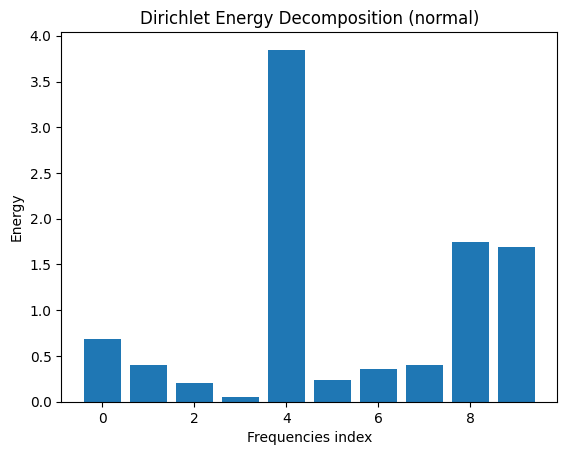
\includegraphics[width=1\linewidth]{images/energy1.png}
\end{subfigure}%
\begin{subfigure}{.33\textwidth}
  \centering
  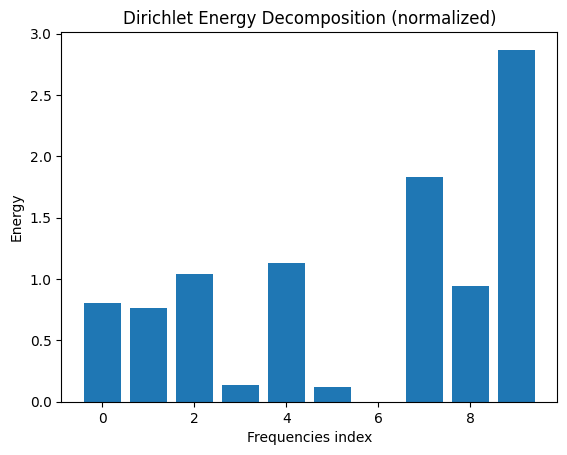
\includegraphics[width=1\linewidth]{images/energy2.png}
\end{subfigure}%
\begin{subfigure}{.33\textwidth}
  \centering
  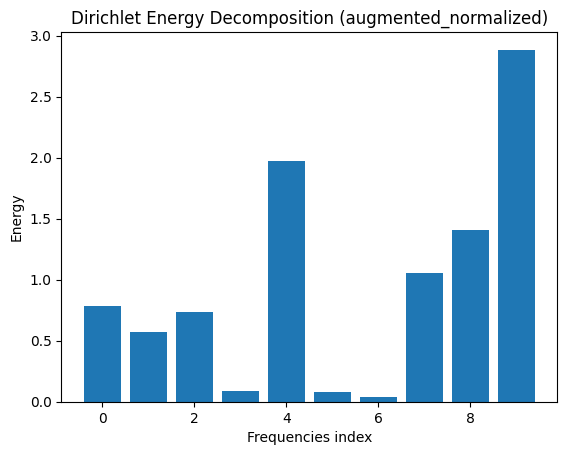
\includegraphics[width=1\linewidth]{images/energy3.png}
\end{subfigure}%
\caption{Energy Decomposition by frequencies of a Erdos-Rényi random graph. The Laplacian used is respectively $\Delta$, $\Bar{\Delta}$ and $\Tilde{\Delta}$}
\end{figure}

We also proved that the Dirichlet energy converges to 0 for the isotropic diffusion. As a use case, we will consider the dynamics of the normal Laplacian $\Delta$:
$$
\dot{X}(t) = -\Delta X(t)
$$

\begin{figure}[h!]
\centering
\begin{subfigure}{.5\textwidth}
  \centering
  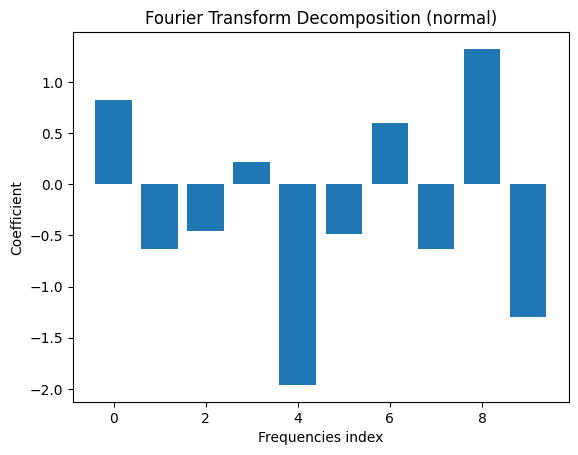
\includegraphics[width=1\linewidth]{images/ft-t1.png}
\end{subfigure}%
\begin{subfigure}{.5\textwidth}
  \centering
  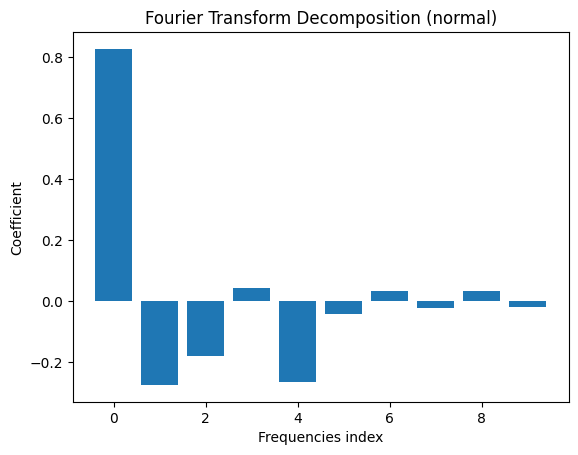
\includegraphics[width=1\linewidth]{images/ft-t2.png}
\end{subfigure}
\begin{subfigure}{.5\textwidth}
  \centering
  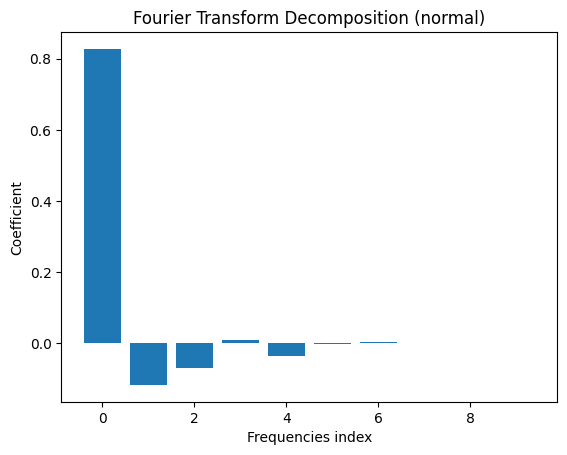
\includegraphics[width=1\linewidth]{images/ft-t3.png}
\end{subfigure}%
\begin{subfigure}{.5\textwidth}
  \centering
  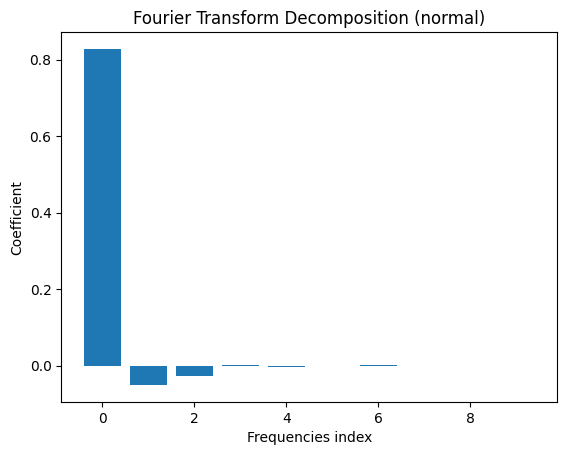
\includegraphics[width=1\linewidth]{images/ft-t4.png}
\end{subfigure}%
\caption{Fourier decomposition of $X(0)$, $X(3.3)$, $X(6.6)$ and $X(10)$}
\end{figure}

\newpage
As we can see, the isotropic diffusion acts as a high-frequency filter on the signal $X$.\\

In practice, to reduce over-smoothing, we can say that two vertices interact if and only if they are very similar and if two vertices are very different we don't want them to interact together:
$$
M(X(t))_{i,j} = \dfrac{1}{1 + \left| \left | X_i(t) - X_j(t) \right| \right|_2^2}
$$

\begin{figure}
\centering
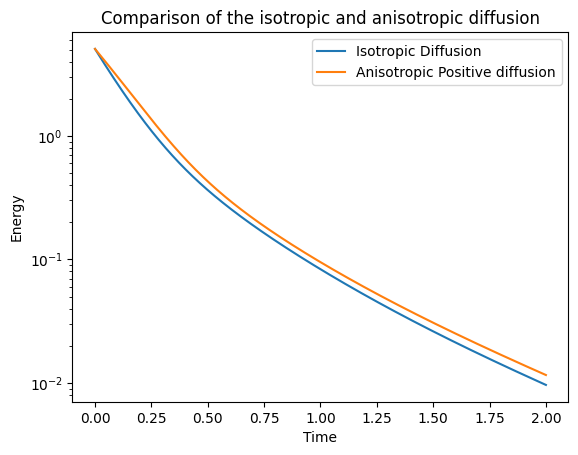
\includegraphics[width=0.7\linewidth]{images/isovsani.png}
\caption{Comparison of the evolution of the Dirichlet Energy for isotropic and anisotropic positive diffusion.}
\label{fig:isovsani}
\end{figure}

However, when running this diffusion process on a random graph we obtain the results of Figure \ref{fig:isovsani}.\\

We can apply theorem \ref{anipos} to indeed prove that even in this case over-smoothing occurs. First let show that under the diffusion $\dot{X}(t) = - div(M(X(t))\nabla X(t))$ the solution $t \mapsto X(t)$ is bounded for the $\left| \left| . \right| \right|_2$ norm:

\begin{align*}
    \dfrac{d \left| \left| X(t) \right| \right|_2^2 }{dt} &= \dfrac{\left<X(t),X(t)\right>}{dt} \\
    &= 2 \left<X(t),\dot{X}(t)\right> \\
    &= -2 \left<X(t),\Delta_{M(X(t))}X(t)\right> \\
    &= -2 E^2_{\Delta_{M(X(t))}}(X(t))
    \leq 0
\end{align*}

Hence, because the $\left| \left| . \right| \right|_2$ norm is bounded, we can find $\varepsilon > 0$, such that for all $i,j \in \{1,...,V\}$:
$$
\dfrac{1}{1 + \left| \left | X_i(t) - X_j(t) \right| \right|_2^2} > \epsilon
$$

We can now apply theorem \ref{anipos} and see that the Dirichlet Energy of $X(t)$ converge exponentially fast to $0$.\\

\newpage
\printbibliography

\end{document}
